\chapter{The ALICE TPC}
\section{Overview}
The ALICE TPC [cite TPC paper] is a gas filled, cylindrical volume with a central cathode and readout anodes on the endplates to apply an electrical field. Due to this field electron ion pairs created by a traversing ionizing particle drift towards the anode and cathode, respectively. The electrons are called primary electrons. Because of their mass, the drift velocity of the electrons is approximately 1000 times higher than the velocity of the ions. At their arrival the electrons induce signals in the segmented anode. This segmentation allows for localisation of the approaching electron on the readout anode. Combining this position with the electron drift time one can reconstruct the point of ionization in three dimensions. Thus, a full 3D-tracking of ionizing particles can be realised with the TPC. When the TPC is placed inside a magnetic field particle trajectories describe helices with a radius proportional to the charge, mass, and velocity of the particles. Using the time-of-flight (TOF) measurement to identify the velocity one can calculate the mass of the particle.\\
The TPC is shown in figure \ref{fig:tpc_sketch}. It features 18 sectors on every endplate, where they are divided into Inner ReadOut Chamber (IROC) and Outer ReadOut Chamber (OROC). Overall there are 72 readout chambers, which are currently based on MWPCs.  
\begin{figure}[]
	%\begin{minipage}[c]{\textwidth}
		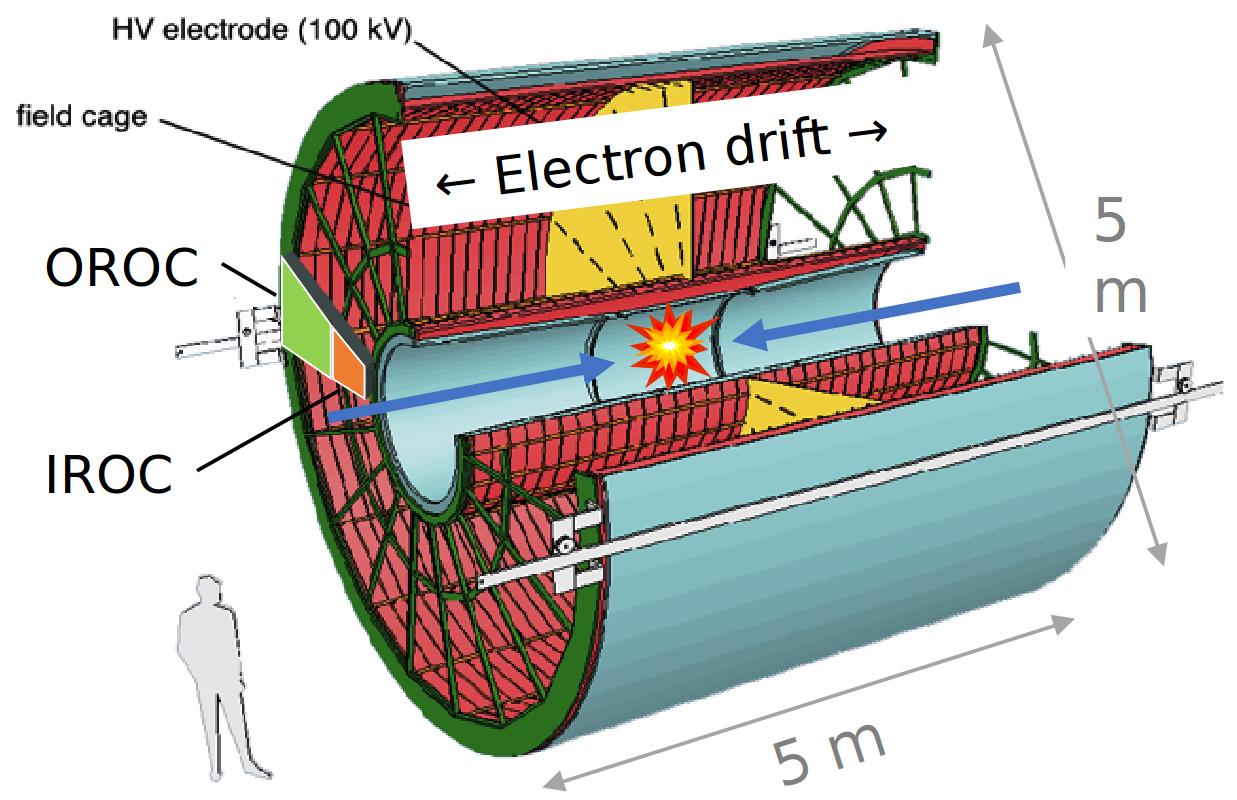
\includegraphics[width=\textwidth]{pictures/ALICE_TPC_scheme.png}
	%\end{minipage}\hfill
	%\begin{minipage}[c]{\textwidth}
		\caption{Scheme of the ALICE TPC with the interaction point in the center. Two readout chambers are shown on top of the support wheel (dark green) building the endplates.}
		\label{fig:tpc_sketch}
	%\end{minipage}
\end{figure}
\section{Operation with MWPCs}
\subsection{Working principle}
Particles produced in collisions pass through the gas volume of the TPC and generate electron ion pairs upon impact ionization. Since in average only one to two electron ion pairs are produced in each collision of the traversing particle with a gas molecule, the induced signal at the anode is not high enough to be observed by the readout electronics. Hence the electrons have to be multiplied. In conventional TPCs MWPCs [cite MWPC] are used for that purpose. MWPCs consist of at least two layers of wires parallel to the anode. The layer closer to the anode is the anode wire grid followed by the cathode wire grid (see fig. \ref{fig: MWPC_fieldlines}). Potentials are applied to the grids in a way that very high fields are reached at the anode wires in order to create electron avalanches by arriving primary electrons. While the electrons drift towards the anode wires and do not contribute to the signal, the ions created in this process drift towards the cathode wires and create mirror charges in the anode. These mirror charges induce a signal which can be read out. While most of the ions reach the cathode wires a significant amount of ions can infringe on the active area of the TPC and drift towards the cathode. This process is called ion back flow. Those ions distort the drift field by building up space charges. However a homogeneous drift field is mandatory to measure the correct drift time and impact point of electrons at the anode to reconstruct the proper trajectory of particles traversing the TPC. To reduce the amount of ions drifting into the active volume, a third layer of wires, the gating grid, is placed above the cathode wires. This gating grid can be enabled by applying a potential in a way that all field lines end on the wires of the gating grid. This forces the ions produced in the avalanche to drift towards the gating grid where they are neutralised. After all ions have reached the gating grid, it is disabled. When the gating grid is disabled it is transparent for electrons but when it is enabled, no electrons can reach the amplification area hence the detector is blind during this time. Therefore, the gating grid limits the detection rate. In case of the ALICE TPC the readout rate is limited to \SI{3.5}{\kilo\hertz} for pp collisions. However, with the high interaction rates after the high luminosity upgrade of the LHC a continuous readout is needed so the gated MWPC is not an option anymore.  
\begin{center}
\begin{figure}[h!]
\centering
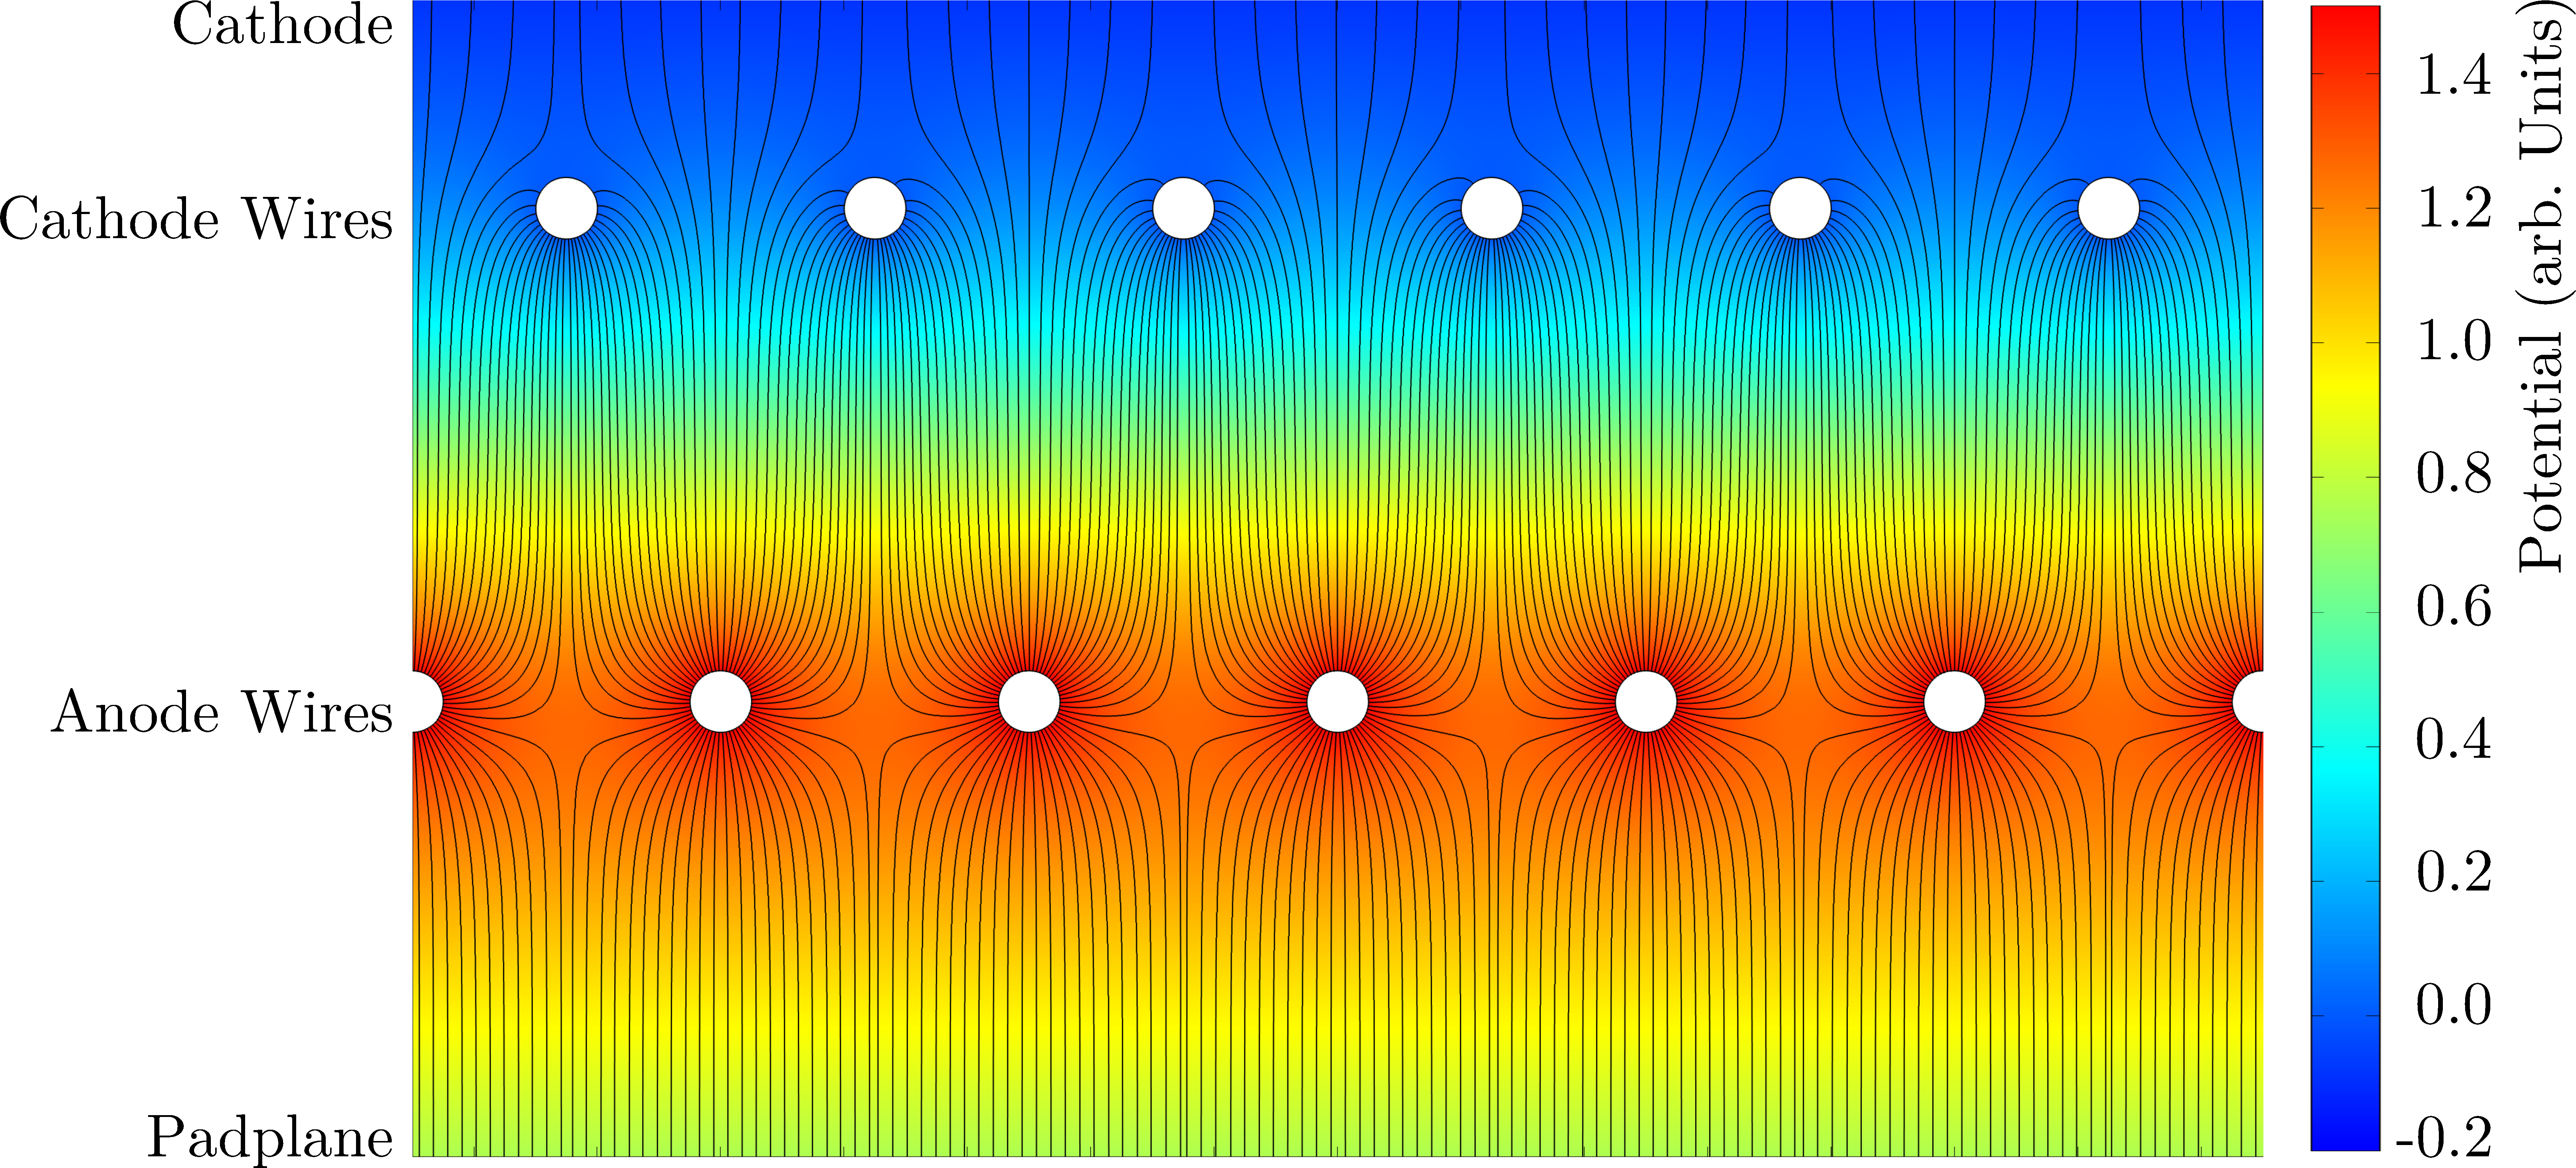
\includegraphics[width=0.8\columnwidth]{pictures/MWPC_fieldlines.pdf}
\caption{Exemplary potential configuration in a MWPC. The field lines are depicted in black, the cross section of the wires is white and the potential is colored [cite Martin]}
\label{fig: MWPC_fieldlines}
\end{figure}
\end{center} 

\subsection{Performance}

\begin{center}
\begin{figure}
\centering
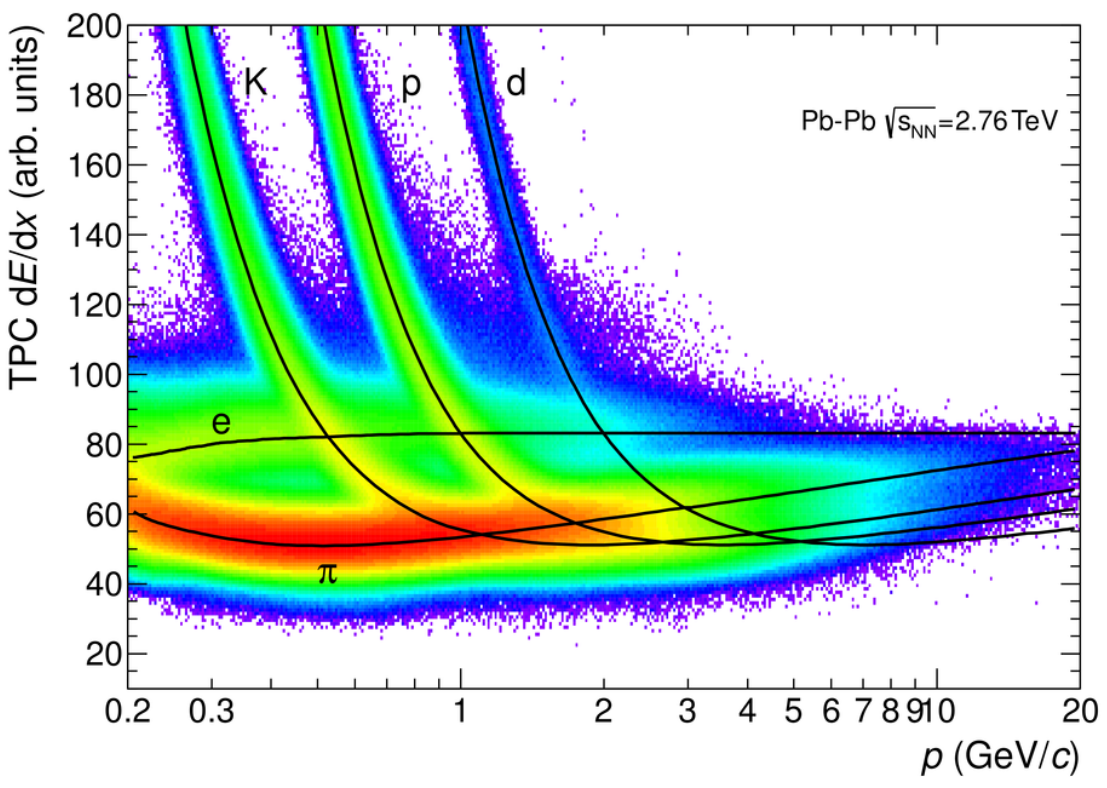
\includegraphics[width=0.8\columnwidth]{pictures/TPC_performance.png}
\caption{Mean energy loss as a function of particle momentum, showing the particle identification performance of the TPC for different particles.}
\label{fig: MWPC_fieldlines}
\end{figure}
\end{center}

\section{Gas Electron Multipliers}
The limitations coming with the use of MWPC-based readout have to be overcome by introducing a new technology. Gas Electron Multipliers (GEM) are the chosen devices since they provide intrinsic ion back flow reduction, and therefore make the installation of a rate limiting gating grid obsolete. A GEM foil [cite Sauli] consists of an insulator foil (thickness: \SI{50}{\micro\meter}) clad with copper on both sides. As insulator material Kapton is often used. By electrochemical etching, the foil is perforated with a regular pattern of conically shaped holes. The perforated area is called active area. Fig. \ref{fig: GEM_dimensions} shows the dimensions of a standard GEM foil. 
\begin{center}
\begin{figure}[]
\centering
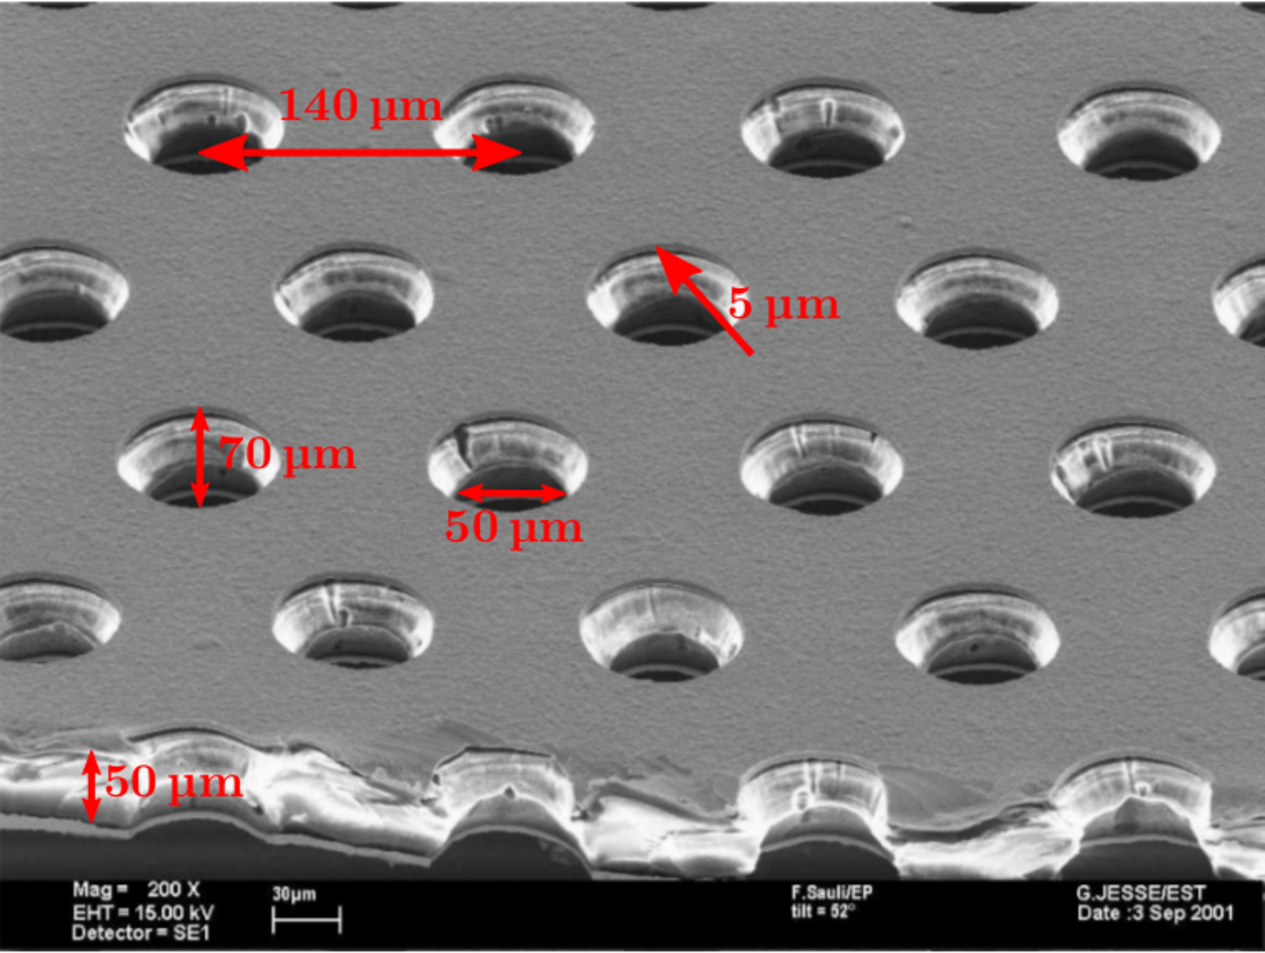
\includegraphics[width=0.8\columnwidth]{pictures/GEM_dimensions.pdf}
\caption{Dimensions of a standard GEM foil}
\label{fig: GEM_dimensions}
\end{figure}
\end{center} 
\subsection{Electron amplification}
By applying a potential difference of several hundred volts between the two copper layers, an electric field in the order of \SI{1000}{\volt\per\centi\meter} can be reached inside the holes. When a GEM foil is placed inside the electric field of a TPC, and the voltages are set properly, a field configuration as shown in fig. \ref{fig: GEM_fieldlines} ensues. The primary electrons drift towards the upper side of the GEM where they are collected into the holes and avalanche amplification appears due to the high field strength inside the holes. Then the electrons are extracted from the bottom side of the GEM and can be accelerated either towards another GEM foil for further amplification or towards the anode for readout. By using more than one GEM an effective gain in the order of $10^4$ can easily be reached. The big asset of GEMs, the intrinsic ion back flow reduction, emerges when it is operated in an asymmetric field where the electric field below the GEM is stronger than above the GEM. In this case some of the field lines end on the top side of the GEM (see fig. \ref{fig: GEM_fieldlines}), forcing a significant amount of the ions created in the avalanche to drift towards the upper surface of the foil where they are neutralized. Therefore, they can not penetrate the drift volume and do not distort the drift field.
\begin{center}
\begin{figure}[]
\centering
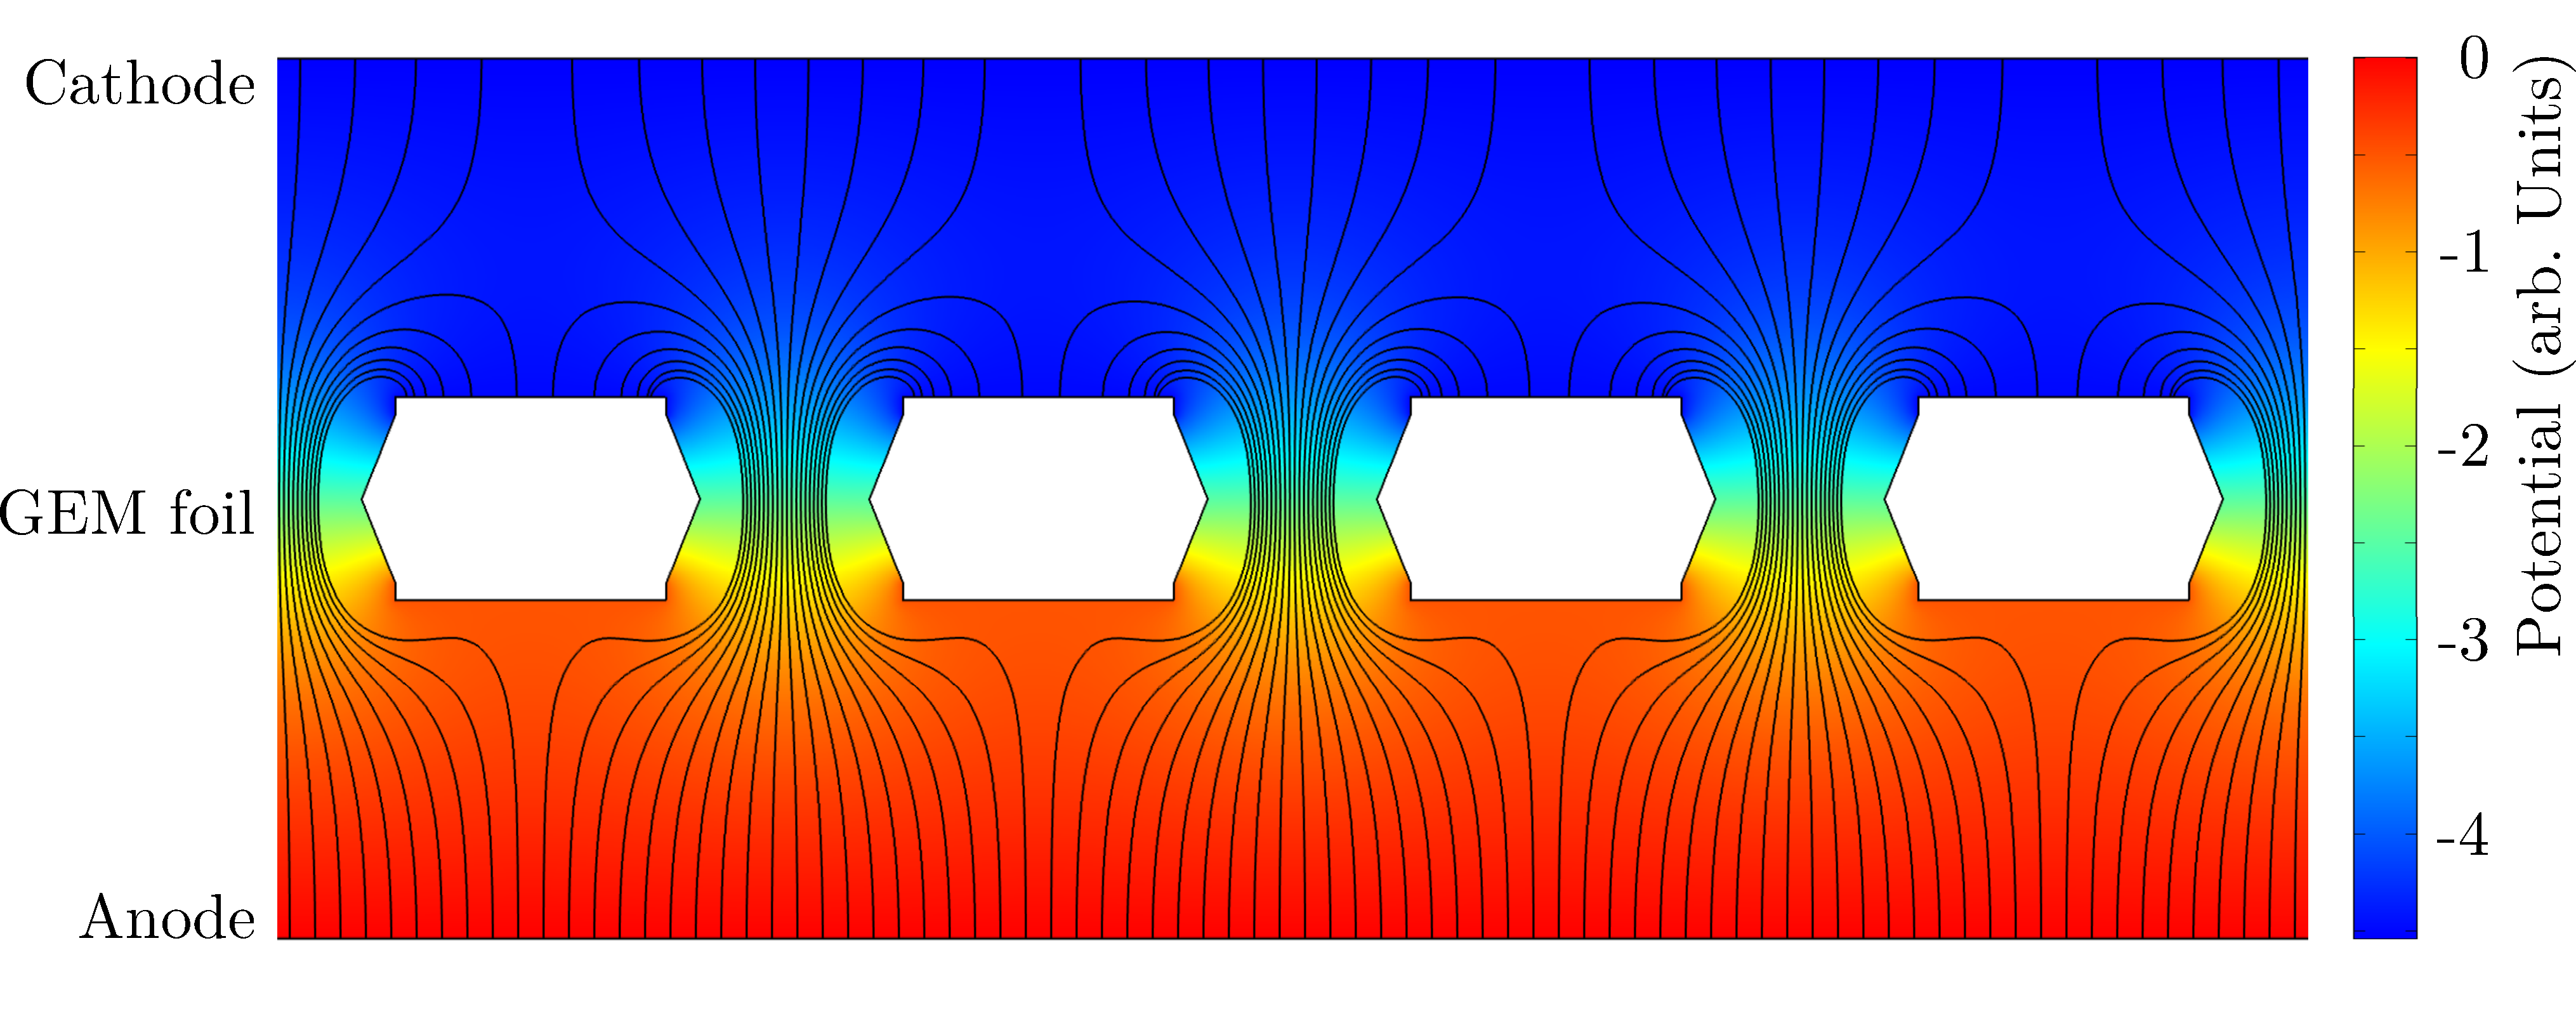
\includegraphics[width=0.8\columnwidth]{pictures/GEM_fieldlines.pdf}
\caption{Exemplary potential configuration of a GEM foil. The field lines are depicted in black, the cross section of the GEM foil is white and the potential is colored [cite Martin]}
\label{fig: GEM_fieldlines}
\end{figure}
\end{center} 
\subsection{Characterisation}
\section{Operation with GEMs}
The TPC operation with GEMs is very different from the MWPC-based TPC. While nothing changes in the creation of primary electrons, the signal creation is fundamentally differs. To reach the required energy loss resolution and ion back flow, a stack of 4 GEMs is choosen to be used for the ALICE TPC.
\subsection{Working principle}
As in the case of the MWPC-based TPC, ionizing particles create electron-ion pairs that are separated by the drift field. The ions drift towards the cathode while the electrons drift towards the amplification stage, which is now a GEM stack. The electrons move inside the GEM holes with a certain collection efficiency and get multiplied trough avalance amplification. Again, the newly created ions drift towards the cathode in backwards direction and the electrons are drawn towards the next GEM, where they are further amplified. This repeats until the electrons have been extracted from the GEM closest to the readout anode. There the electrons dirft towards the anode and induce a signal with negative polarity in contrast to the signal with positive polarity that is induced by the ions in MWPC-based readout. 
\subsection{Performance}